% Options for packages loaded elsewhere
% Options for packages loaded elsewhere
\PassOptionsToPackage{unicode}{hyperref}
\PassOptionsToPackage{hyphens}{url}
%
\documentclass[
  ignorenonframetext,
  aspectratio=169,
]{beamer}
\newif\ifbibliography
\usepackage{pgfpages}
\setbeamertemplate{caption}[numbered]
\setbeamertemplate{caption label separator}{: }
\setbeamercolor{caption name}{fg=normal text.fg}
\beamertemplatenavigationsymbolsempty
% remove section numbering
\setbeamertemplate{part page}{
  \centering
  \begin{beamercolorbox}[sep=16pt,center]{part title}
    \usebeamerfont{part title}\insertpart\par
  \end{beamercolorbox}
}
\setbeamertemplate{section page}{
  \centering
  \begin{beamercolorbox}[sep=12pt,center]{section title}
    \usebeamerfont{section title}\insertsection\par
  \end{beamercolorbox}
}
\setbeamertemplate{subsection page}{
  \centering
  \begin{beamercolorbox}[sep=8pt,center]{subsection title}
    \usebeamerfont{subsection title}\insertsubsection\par
  \end{beamercolorbox}
}
% Prevent slide breaks in the middle of a paragraph
\widowpenalties 1 10000
\raggedbottom
\usepackage{iftex}
\ifPDFTeX
  \usepackage[T1]{fontenc}
  \usepackage[utf8]{inputenc}
  \usepackage{textcomp} % provide euro and other symbols
\else % if luatex or xetex
  \usepackage{unicode-math} % this also loads fontspec
  \defaultfontfeatures{Scale=MatchLowercase}
  \defaultfontfeatures[\rmfamily]{Ligatures=TeX,Scale=1}
\fi
\usepackage{lmodern}

\usetheme[]{metropolis}
\ifPDFTeX\else
  % xetex/luatex font selection
\fi
% Use upquote if available, for straight quotes in verbatim environments
\IfFileExists{upquote.sty}{\usepackage{upquote}}{}
\IfFileExists{microtype.sty}{% use microtype if available
  \usepackage[]{microtype}
  \UseMicrotypeSet[protrusion]{basicmath} % disable protrusion for tt fonts
}{}
\makeatletter
\@ifundefined{KOMAClassName}{% if non-KOMA class
  \IfFileExists{parskip.sty}{%
    \usepackage{parskip}
  }{% else
    \setlength{\parindent}{0pt}
    \setlength{\parskip}{6pt plus 2pt minus 1pt}}
}{% if KOMA class
  \KOMAoptions{parskip=half}}
\makeatother


\usepackage{longtable,booktabs,array}
\usepackage{calc} % for calculating minipage widths
\usepackage{caption}
% Make caption package work with longtable
\makeatletter
\def\fnum@table{\tablename~\thetable}
\makeatother
\usepackage{graphicx}
\makeatletter
\newsavebox\pandoc@box
\newcommand*\pandocbounded[1]{% scales image to fit in text height/width
  \sbox\pandoc@box{#1}%
  \Gscale@div\@tempa{\textheight}{\dimexpr\ht\pandoc@box+\dp\pandoc@box\relax}%
  \Gscale@div\@tempb{\linewidth}{\wd\pandoc@box}%
  \ifdim\@tempb\p@<\@tempa\p@\let\@tempa\@tempb\fi% select the smaller of both
  \ifdim\@tempa\p@<\p@\scalebox{\@tempa}{\usebox\pandoc@box}%
  \else\usebox{\pandoc@box}%
  \fi%
}
% Set default figure placement to htbp
\def\fps@figure{htbp}
\makeatother





\setlength{\emergencystretch}{3em} % prevent overfull lines

\providecommand{\tightlist}{%
  \setlength{\itemsep}{0pt}\setlength{\parskip}{0pt}}



 


% ============================================================
%  Econ 2203 — Beamer Metropolis Theme Preamble
%  Course: International Trade and Policy in Agriculture
%  Instructor: Nithin M, Department of Development Economics
% ============================================================

% MUST be first: load Metropolis theme before \metroset and colour overrides
\usetheme{metropolis}

% Only load packages not already provided by pandoc's beamer template
\usepackage{amsmath,amssymb}

% ---- Brand colours -----------------------------------------
\definecolor{brandblue}{HTML}{012169}
\definecolor{brandgold}{HTML}{B9975B}
\definecolor{lightblue}{HTML}{E8EDF5}

% ---- Metropolis colour overrides ---------------------------
% Main palette
\setbeamercolor{normal text}{fg=black,bg=white}
\setbeamercolor{background canvas}{bg=white}
\setbeamercolor{alerted text}{fg=brandgold}
\setbeamercolor{example text}{fg=brandblue!70!black}

% Title slide
\setbeamercolor{title}{fg=white,bg=brandblue}
\setbeamercolor{subtitle}{fg=brandgold}
\setbeamercolor{author}{fg=white}
\setbeamercolor{institute}{fg=brandgold!80!white}
\setbeamercolor{date}{fg=white}
\setbeamercolor{title page header}{fg=white,bg=brandblue}

% Frametitle bar
\setbeamercolor{frametitle}{fg=white,bg=brandblue}

% Progress bar → gold
\setbeamercolor{progress bar}{fg=brandgold,bg=brandblue!30}
\setbeamercolor{title separator}{fg=brandgold}
\setbeamercolor{progress bar in head/foot}{fg=brandgold,bg=brandblue!20}
\setbeamercolor{progress bar in section page}{fg=brandgold,bg=brandblue!20}

% Blocks
\setbeamercolor{block title}{bg=brandblue,fg=white}
\setbeamercolor{block body}{bg=lightblue,fg=black}
\setbeamercolor{block title alerted}{bg=brandgold,fg=white}
\setbeamercolor{block body alerted}{bg=brandgold!12,fg=black}
\setbeamercolor{block title example}{bg=brandblue!70!black,fg=white}
\setbeamercolor{block body example}{bg=brandblue!8,fg=black}

% Structure / lists
\setbeamercolor{structure}{fg=brandblue}
\setbeamercolor{section in toc}{fg=brandblue}
\setbeamercolor{itemize item}{fg=brandblue}
\setbeamercolor{itemize subitem}{fg=brandgold}
\setbeamercolor{enumerate item}{fg=brandblue}
\setbeamercolor{description item}{fg=brandblue}

% ---- Metropolis options ------------------------------------
\metroset{
  progressbar    = frametitle,   % gold bar under frametitle
  sectionpage    = none,
  numbering      = fraction,
  block          = fill
}

% ---- Fonts (Metropolis uses Fira Sans; fallback gracefully) -
\setbeamerfont{title}{size=\Large,series=\bfseries}
\setbeamerfont{subtitle}{size=\normalsize,series=\mdseries}
\setbeamerfont{frametitle}{size=\large,series=\bfseries}
\setbeamerfont{block title}{size=\normalsize,series=\bfseries}
\setbeamerfont{caption}{size=\footnotesize}

% ---- Footer: course info + slide number --------------------
\setbeamertemplate{footline}{%
  \begin{beamercolorbox}[wd=\paperwidth,ht=2.0ex,dp=1ex]{footline}%
    \hspace{0.8em}%
    {\footnotesize\color{brandblue!60}%
      Econ 2203 \textbar{} International Trade and Policy in Agriculture
      \hfill Nithin M \hfill
      \insertframenumber{}/\inserttotalframenumber\hspace{0.8em}}%
  \end{beamercolorbox}%
}

% ---- Misc --------------------------------------------------
\setlength{\parskip}{2pt}
\setbeamertemplate{navigation symbols}{}

% tighter column sep for side-by-side content
\setlength{\columnsep}{0.8em}

% ---- Max 6 lines per slide: compact list typesetting -------
% Smaller fonts at each list depth
\setbeamerfont{itemize/enumerate body}{size=\small}
\setbeamerfont{itemize/enumerate subbody}{size=\footnotesize}
\setbeamerfont{itemize/enumerate subsubbody}{size=\scriptsize}

% Tight vertical spacing injected at the start of each list level
\setbeamertemplate{itemize/enumerate body begin}{%
  \setlength{\itemsep}{3pt}\setlength{\parsep}{0pt}}
\setbeamertemplate{itemize/enumerate subbody begin}{%
  \setlength{\itemsep}{2pt}\setlength{\parsep}{0pt}}
\setbeamertemplate{itemize/enumerate subsubbody begin}{%
  \setlength{\itemsep}{1pt}\setlength{\parsep}{0pt}}

% Global safety net: default frame shrink = 10 %
% \beamer@shrinkfalse is called ONCE in beamer's frame init (line 438 of
% beamerbaseframe.sty) before the user's options are processed (line 444).
% By redefining it we inject shrink=10 right after the reset; if the frame
% explicitly specifies [shrink=X], the later \setkeys call overrides it.
\makeatletter
\let\beamer@orig@shrinkfalse\beamer@shrinkfalse
\def\beamer@shrinkfalse{%
  \beamer@orig@shrinkfalse
  \setkeys{beamerframe}{shrink=10}}
\makeatother

% Fix: make \label truly robust in moving arguments.
% Quarto wraps figure labels inside captions; Metropolis expands them
% in batchmode causing a crash. DeclareRobustCommand prevents expansion.
\makeatletter
\let\quarto@originallabel\label
\DeclareRobustCommand*{\label}[1]{\quarto@originallabel{#1}}
\makeatother

% Prevent figures from overflowing Beamer frames.
% width=\linewidth: scale to text width (already Quarto default);
% height=0.6\textheight: cap height so figures never push past the frame bottom.
% keepaspectratio: never distort — whichever constraint binds first wins.
\setkeys{Gin}{width=\linewidth,height=0.55\textheight,keepaspectratio}
\makeatletter
\@ifpackageloaded{caption}{}{\usepackage{caption}}
\AtBeginDocument{%
\ifdefined\contentsname
  \renewcommand*\contentsname{Table of contents}
\else
  \newcommand\contentsname{Table of contents}
\fi
\ifdefined\listfigurename
  \renewcommand*\listfigurename{List of Figures}
\else
  \newcommand\listfigurename{List of Figures}
\fi
\ifdefined\listtablename
  \renewcommand*\listtablename{List of Tables}
\else
  \newcommand\listtablename{List of Tables}
\fi
\ifdefined\figurename
  \renewcommand*\figurename{Figure}
\else
  \newcommand\figurename{Figure}
\fi
\ifdefined\tablename
  \renewcommand*\tablename{Table}
\else
  \newcommand\tablename{Table}
\fi
}
\@ifpackageloaded{float}{}{\usepackage{float}}
\floatstyle{ruled}
\@ifundefined{c@chapter}{\newfloat{codelisting}{h}{lop}}{\newfloat{codelisting}{h}{lop}[chapter]}
\floatname{codelisting}{Listing}
\newcommand*\listoflistings{\listof{codelisting}{List of Listings}}
\makeatother
\makeatletter
\makeatother
\makeatletter
\@ifpackageloaded{caption}{}{\usepackage{caption}}
\@ifpackageloaded{subcaption}{}{\usepackage{subcaption}}
\makeatother

\usepackage{bookmark}
\IfFileExists{xurl.sty}{\usepackage{xurl}}{} % add URL line breaks if available
\urlstyle{same}
\hypersetup{
  pdftitle={Lecture 10: India's External Sector},
  pdfauthor={Nithin M},
  hidelinks,
  pdfcreator={LaTeX via pandoc}}


\title{Lecture 10: India's External Sector}
\subtitle{Econ 2203 \textbar{} International Trade and Policy in
Agriculture}
\author{Nithin M}
\date{2026-06-27}
\institute{Department of Development Economics}

\begin{document}
\frame{\titlepage}


\begin{frame}{India's External Sector}
\phantomsection\label{indias-external-sector}
A deep dive into India's trade structure, agricultural trade, and
balance of payments
\end{frame}

\begin{frame}{Overview of India's External Sector}
\phantomsection\label{overview-of-indias-external-sector}
\begin{columns}[T]
\begin{column}{0.6\linewidth}
India is a \textbf{major trading nation} --- ranked among the top 20
exporters and importers globally.

Key FY2024 aggregates:

\begin{itemize}
\tightlist
\item
  \textbf{Merchandise exports:} \$437 billion
\item
  \textbf{Merchandise imports:} \$677 billion
\item
  \textbf{Trade deficit:} −\$240 billion
\item
  \textbf{Services exports:} \$338 billion
\item
  \textbf{Remittances:} \$120 billion
\end{itemize}
\end{column}

\begin{column}{0.4\linewidth}
\textbf{Why does this matter for agriculture?}

India's external sector shapes:

\begin{itemize}
\tightlist
\item
  Price of edible oils (imports)
\item
  Farmer income (export demand)
\item
  Food inflation (rupee/import costs)
\item
  BoP sustainability
\end{itemize}
\end{column}
\end{columns}
\end{frame}

\begin{frame}{Merchandise Exports: Structure FY2024}
\phantomsection\label{merchandise-exports-structure-fy2024}
\textbf{Top 5 Merchandise Export Categories --- FY2024}

\begin{longtable}[]{@{}lll@{}}
\toprule\noalign{}
Category & Value (USD B) & Share of Total \\
\midrule\noalign{}
\endhead
Engineering goods & \$109 & 14.0\% \\
Petroleum products & \$96 & 12.3\% \\
\textbf{Agriculture \& allied} & \textbf{\$43.7} & \textbf{5.6\%} \\
Gems \& jewellery & \$37 & 4.8\% \\
Chemicals & \$32 & 4.1\% \\
\textbf{Total merchandise} & \textbf{\$437} & \\
\bottomrule\noalign{}
\end{longtable}

Agriculture contributes \textasciitilde5.6\% of total merchandise
exports --- a modest but strategically important share.
\end{frame}

\begin{frame}{Merchandise Export Composition: FY2024}
\phantomsection\label{merchandise-export-composition-fy2024}
\begin{figure}

\centering{

\pandocbounded{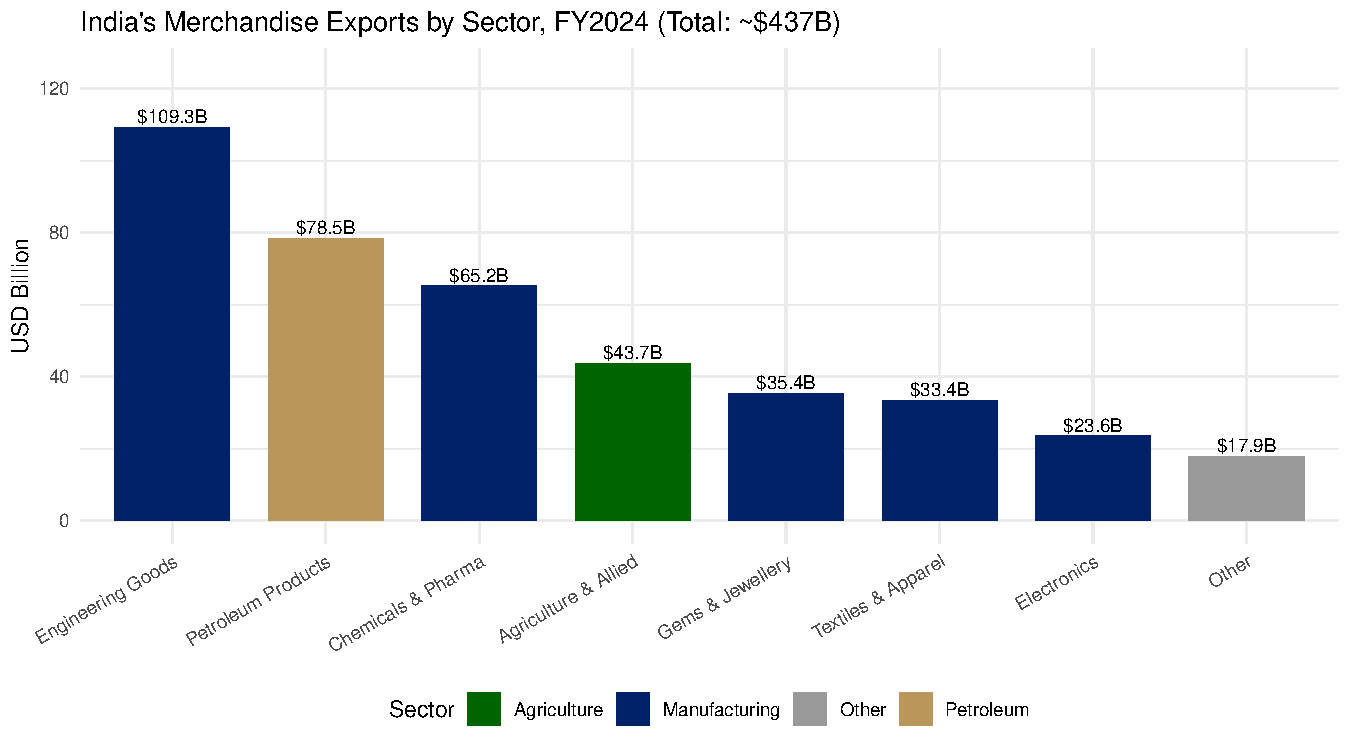
\includegraphics[keepaspectratio]{Lecture10_India_External_Sector_files/figure-beamer/fig-export-composition-1.pdf}}

}

\caption{India's Merchandise Export
Composition, FY2024 (USD billion) Source: DGCI\&S / Ministry of Commerce
and Industry, GoI.}
\label{fig-export-composition}

\end{figure}%

Engineering goods (\$109B) dominate --- India's shift toward capital
goods exports. Agriculture (\$44B) is the 5th largest category, but
holds outsized strategic importance for rural incomes and food security
diplomacy.
\end{frame}

\begin{frame}{Merchandise Imports: Structure FY2024}
\phantomsection\label{merchandise-imports-structure-fy2024}
\begin{columns}[T]
\begin{column}{0.55\linewidth}
\textbf{Top Import Categories:}

\begin{longtable}[]{@{}ll@{}}
\toprule\noalign{}
Category & USD B \\
\midrule\noalign{}
\endhead
Petroleum \& crude oil & \$232 \\
Engineering goods & \$91 \\
Electronic goods & \$80 \\
Gold & \$47 \\
\textbf{Edible oils} & \textbf{\$14} \\
Pulses & \$2.8 \\
\bottomrule\noalign{}
\end{longtable}
\end{column}

\begin{column}{0.45\linewidth}
\textbf{Agricultural import vulnerability}

Edible oils at \$14B represent a structural dependency --- India imports
\textasciitilde60--65\% of its edible oil needs.

This is India's single largest agricultural import burden.
\end{column}
\end{columns}
\end{frame}

\begin{frame}{Merchandise Import Composition: FY2024}
\phantomsection\label{merchandise-import-composition-fy2024}
\begin{figure}

\centering{

\pandocbounded{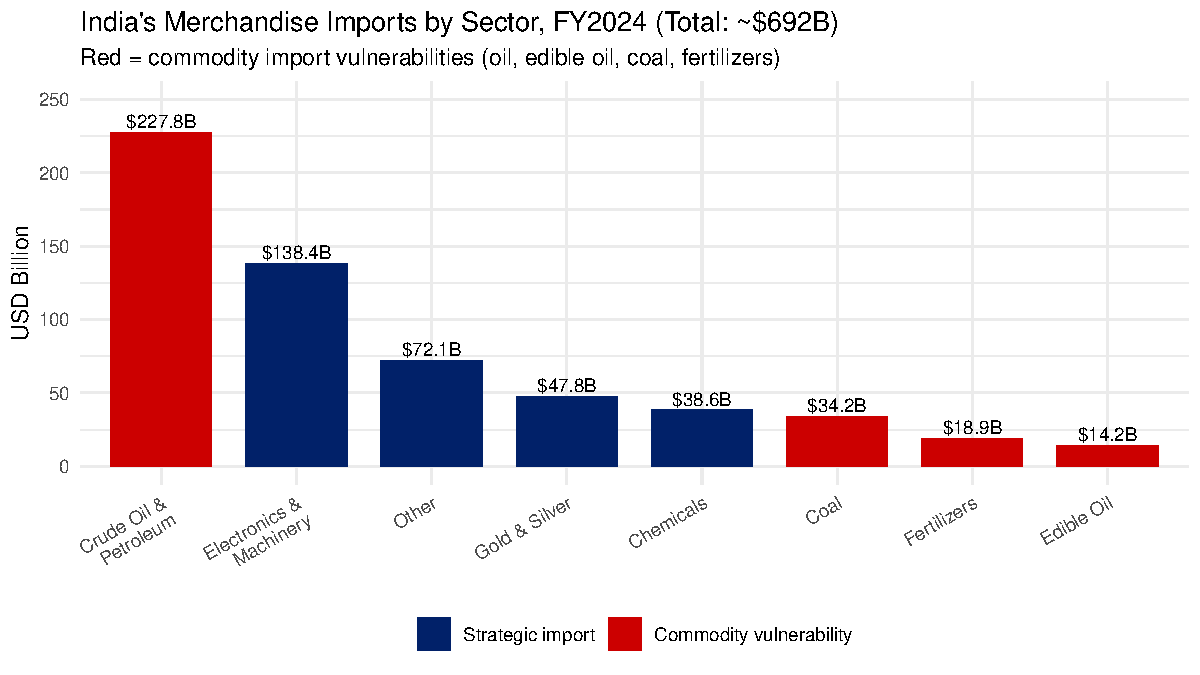
\includegraphics[keepaspectratio]{Lecture10_India_External_Sector_files/figure-beamer/fig-import-composition-1.pdf}}

}

\caption{India's Merchandise Import
Composition, FY2024 (USD billion) Source: DGCI\&S / Ministry of Commerce
and Industry, GoI.}
\label{fig-import-composition}

\end{figure}%

\textbf{Vulnerability arithmetic:} Crude oil (\$228B) + Coal (\$34B) +
Fertilizers (\$19B) + Edible oil (\$14B) = \textbf{\textasciitilde\$295B
in commodity imports} --- 43\% of total imports are subject to global
commodity price shocks beyond India's control.
\end{frame}

\begin{frame}{Agricultural Exports FY2024: Breakdown}
\phantomsection\label{agricultural-exports-fy2024-breakdown}
\textbf{India's total agricultural exports FY2024: \textasciitilde\$43.7
billion}

\begin{columns}[T]
\begin{column}{0.5\linewidth}
\begin{longtable}[]{@{}ll@{}}
\toprule\noalign{}
Commodity & USD B \\
\midrule\noalign{}
\endhead
Marine products & \$7.6 \\
\textbf{Non-basmati rice} & \textbf{\$6.4} \\
Basmati rice & \$5.8 \\
Processed food & \$4.8 \\
\bottomrule\noalign{}
\end{longtable}
\end{column}

\begin{column}{0.5\linewidth}
\begin{longtable}[]{@{}ll@{}}
\toprule\noalign{}
Commodity & USD B \\
\midrule\noalign{}
\endhead
Spices & \$3.7 \\
Cotton & \$2.7 \\
Coffee & \$1.2 \\
Others & \textasciitilde\$11.5 \\
\bottomrule\noalign{}
\end{longtable}
\end{column}
\end{columns}

⚠️ Non-basmati rice exports were restricted from August 2023,
significantly curtailing export earnings.
\end{frame}

\begin{frame}{Agricultural Imports FY2024: Breakdown}
\phantomsection\label{agricultural-imports-fy2024-breakdown}
\textbf{Total agricultural imports: \textasciitilde\$28.2 billion}

\begin{columns}[T]
\begin{column}{0.55\linewidth}
\textbf{Edible Oils --- \$14 billion (largest component)}

\begin{longtable}[]{@{}ll@{}}
\toprule\noalign{}
Oil & USD B \\
\midrule\noalign{}
\endhead
Palm oil & \$9.5 \\
Soybean oil & \$2.5 \\
Sunflower oil & \$2.0 \\
\bottomrule\noalign{}
\end{longtable}
\end{column}

\begin{column}{0.45\linewidth}
\textbf{Other major imports:}

\begin{itemize}
\tightlist
\item
  Pulses: \textbf{\$2.8B}\\
  \emph{(Canada, Australia key sources)}
\item
  Fresh fruits: \textbf{\$1.8B}
\item
  Cashew (raw): \textasciitilde\$1.5B
\item
  Spices (for re-export): \textasciitilde\$0.8B
\end{itemize}
\end{column}
\end{columns}
\end{frame}

\begin{frame}{India's Net Agricultural Trade Position}
\phantomsection\label{indias-net-agricultural-trade-position}
\textbf{Agricultural Trade Balance FY2024}

Exports \$43.7B − Imports \$28.2B = \textbf{Surplus +\$15.5B}

\textbf{Five-Year Trend in Agricultural Trade Surplus:}

\begin{longtable}[]{@{}ll@{}}
\toprule\noalign{}
FY & Surplus (USD B) \\
\midrule\noalign{}
\endhead
FY2020 & \$17.0 \\
FY2021 & \$20.0 \\
FY2022 & \$25.0 \\
FY2023 & \$15.8 \\
FY2024 & \$15.5 \\
\bottomrule\noalign{}
\end{longtable}

The sharp drop from FY2022 to FY2023 reflects global commodity price
corrections and India's rice export restrictions.
\end{frame}

\begin{frame}{India's Key Merchandise Trading Partners}
\phantomsection\label{indias-key-merchandise-trading-partners}
\begin{columns}[T]
\begin{column}{0.5\linewidth}
\textbf{Top Export Destinations}

\begin{enumerate}
\tightlist
\item
  🇺🇸 USA --- \$77B
\item
  🇦🇪 UAE --- \$35B
\item
  🇳🇱 Netherlands --- \$23B
\item
  🇬🇧 UK --- \$19B
\item
  🇧🇩 Bangladesh --- \$14B
\end{enumerate}
\end{column}

\begin{column}{0.5\linewidth}
\textbf{Top Import Sources}

\begin{enumerate}
\tightlist
\item
  🇨🇳 China --- \$101B
\item
  🇷🇺 Russia --- \$61B
\item
  🇦🇪 UAE --- \$48B
\item
  🇺🇸 USA --- \$42B
\item
  🇮🇶 Iraq --- \$22B
\end{enumerate}
\end{column}
\end{columns}

\textbf{China dominates imports} --- especially electronics, machinery,
chemicals. India's trade deficit with China alone is
\textasciitilde\$85B. Reducing this is a stated policy goal.
\end{frame}

\begin{frame}{India's Trade Partners: FY2024}
\phantomsection\label{indias-trade-partners-fy2024}
\begin{figure}

\centering{

\pandocbounded{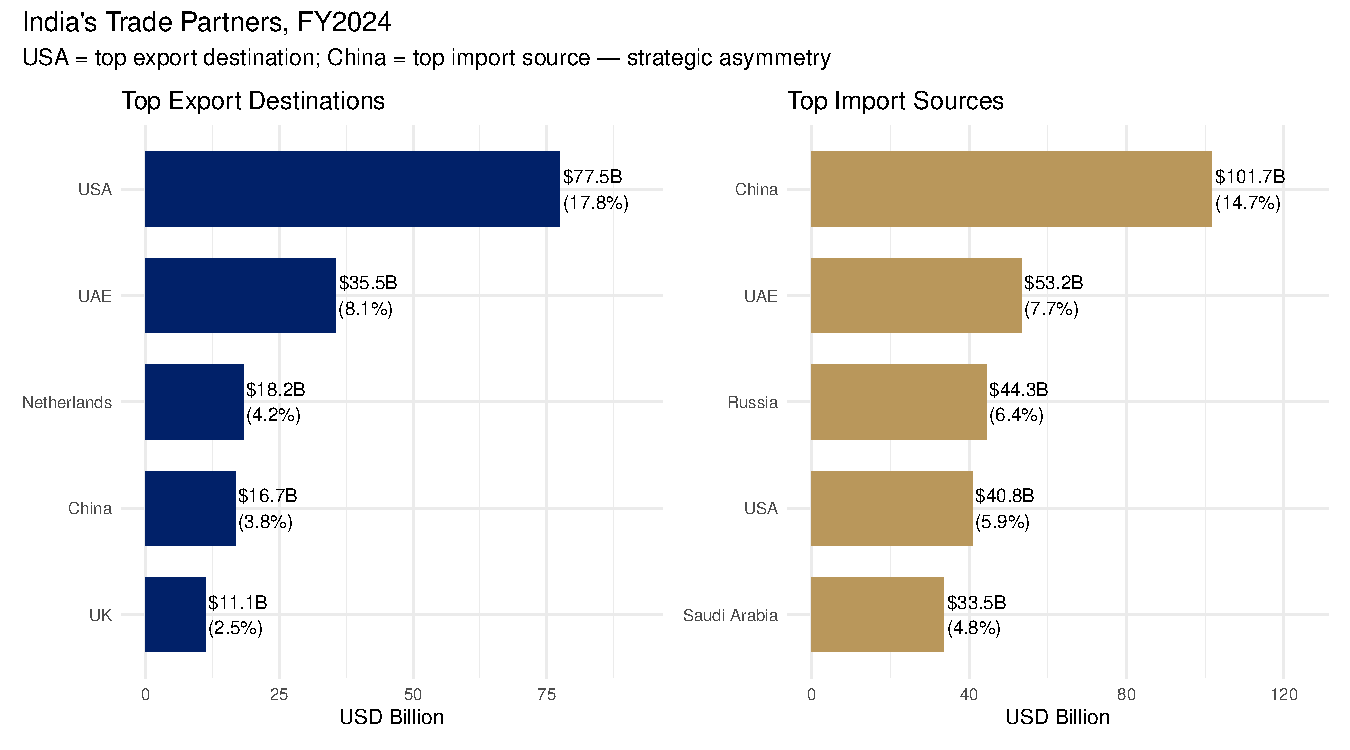
\includegraphics[keepaspectratio]{Lecture10_India_External_Sector_files/figure-beamer/fig-trade-partners-1.pdf}}

}

\caption{India's Top 5 Export Destinations and
Import Sources, FY2024 Source: DGCI\&S / Ministry of Commerce and
Industry, GoI.}
\label{fig-trade-partners}

\end{figure}%

\textbf{Strategic asymmetry:} India exports most to the USA (\$78B) but
imports most from China (\$102B). The bilateral trade deficit with China
alone (\textasciitilde\$85B) exceeds India's entire trade surplus with
the USA.
\end{frame}

\begin{frame}{Agricultural Trade Partners}
\phantomsection\label{agricultural-trade-partners}
\begin{columns}[T]
\begin{column}{0.5\linewidth}
\textbf{Top Agri Export Markets}

\begin{enumerate}
\tightlist
\item
  USA --- marine, spices, processed
\item
  Bangladesh --- rice, food grains
\item
  UAE --- rice, vegetables, spices
\item
  China --- cotton, marine, soybean
\item
  Saudi Arabia --- rice, spices
\end{enumerate}

\emph{Rice dominates exports to South/SE Asia}
\end{column}

\begin{column}{0.5\linewidth}
\textbf{Top Agri Import Sources}

\begin{enumerate}
\tightlist
\item
  Indonesia --- palm oil
\item
  Malaysia --- palm oil
\item
  Canada --- pulses, lentils
\item
  Australia --- pulses, wheat (intermittent)
\item
  Ukraine/Argentina --- sunflower/soybean oil
\end{enumerate}
\end{column}
\end{columns}

India's agricultural trade geography reflects its structural reliance on
SE Asia for edible oils and the Anglosphere for pulses.
\end{frame}

\begin{frame}{Services Exports: The Other Engine}
\phantomsection\label{services-exports-the-other-engine}
\textbf{Services exports FY2024: \$338 billion} --- India's invisible
export superpower

\begin{columns}[T]
\begin{column}{0.55\linewidth}
\begin{longtable}[]{@{}ll@{}}
\toprule\noalign{}
Services Category & USD B \\
\midrule\noalign{}
\endhead
IT/Software services & \$220 \\
Business process mgmt & \$38 \\
Financial services & \$20 \\
Travel \& tourism & \$18 \\
Other services & \$42 \\
\bottomrule\noalign{}
\end{longtable}
\end{column}

\begin{column}{0.45\linewidth}
\textbf{Why this matters for agri trade:}

IT export earnings provide forex that finances agricultural imports
(edible oils, pulses).

Without IT services surplus, India's BoP position would be far more
stressed.
\end{column}
\end{columns}
\end{frame}

\begin{frame}{Services Trade Composition: FY2024}
\phantomsection\label{services-trade-composition-fy2024}
\begin{figure}

\centering{

\pandocbounded{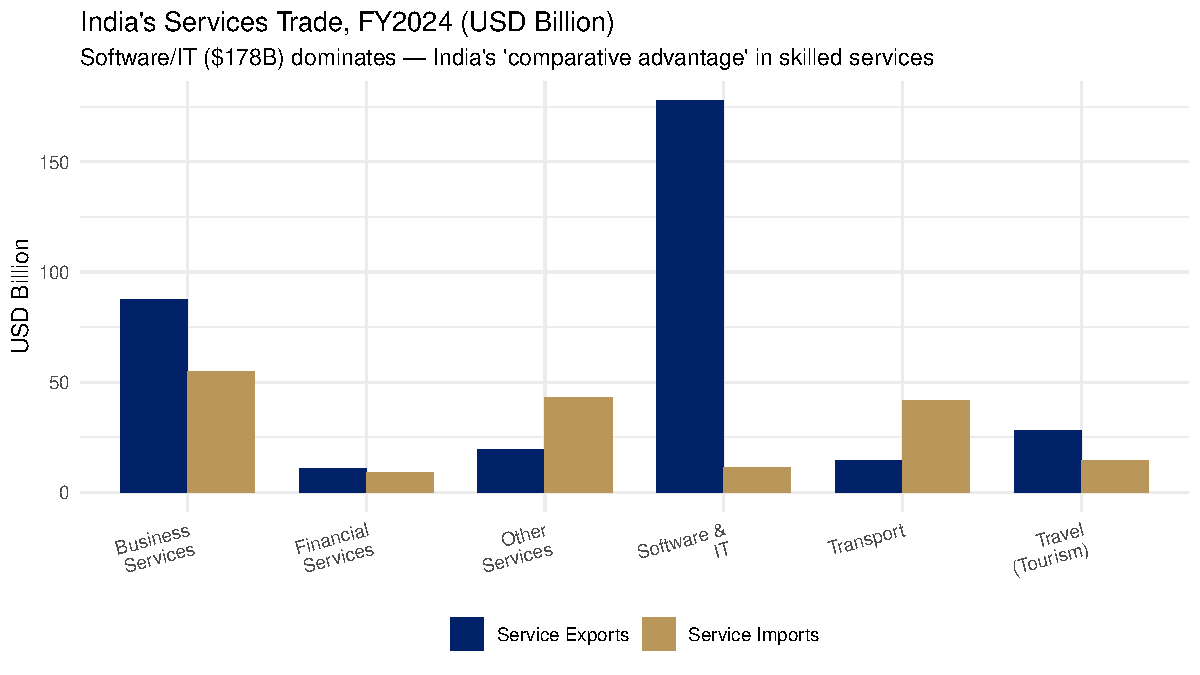
\includegraphics[keepaspectratio]{Lecture10_India_External_Sector_files/figure-beamer/fig-services-trade-1.pdf}}

}

\caption{India's Services Trade Composition,
FY2024 (USD billion) Source: RBI, Balance of Payments Statistics.}
\label{fig-services-trade}

\end{figure}%

\textbf{Revealed comparative advantage:} India's RCA in Software/IT
services is extremely high --- the \$194B export vs \$12B import
reflects a structural specialisation that offsets the entire merchandise
trade deficit (\$76B) by itself.
\end{frame}

\begin{frame}{Remittances: India's Hidden BoP Pillar}
\phantomsection\label{remittances-indias-hidden-bop-pillar}
\begin{columns}[T]
\begin{column}{0.6\linewidth}
\textbf{India is the world's largest recipient of remittances}

\begin{itemize}
\tightlist
\item
  FY2024 inflows: \textbf{\$120 billion}
\item
  Share of GDP: \textasciitilde3.4\%
\item
  Primary sources: Gulf countries (UAE, Saudi Arabia, Kuwait), USA, UK,
  Canada
\end{itemize}

\textbf{Key sending states:} Kerala, UP, Bihar, Rajasthan, Punjab
\end{column}

\begin{column}{0.4\linewidth}
\textbf{Remittances vs Trade Deficit}

Trade deficit: −\$76B\\
Remittances: +\$120B

Remittances alone more than offset the merchandise trade deficit --- a
critical BoP stabilizer.
\end{column}
\end{columns}
\end{frame}

\begin{frame}{Remittances: Global Comparison}
\phantomsection\label{remittances-global-comparison}
\begin{figure}

\centering{

\pandocbounded{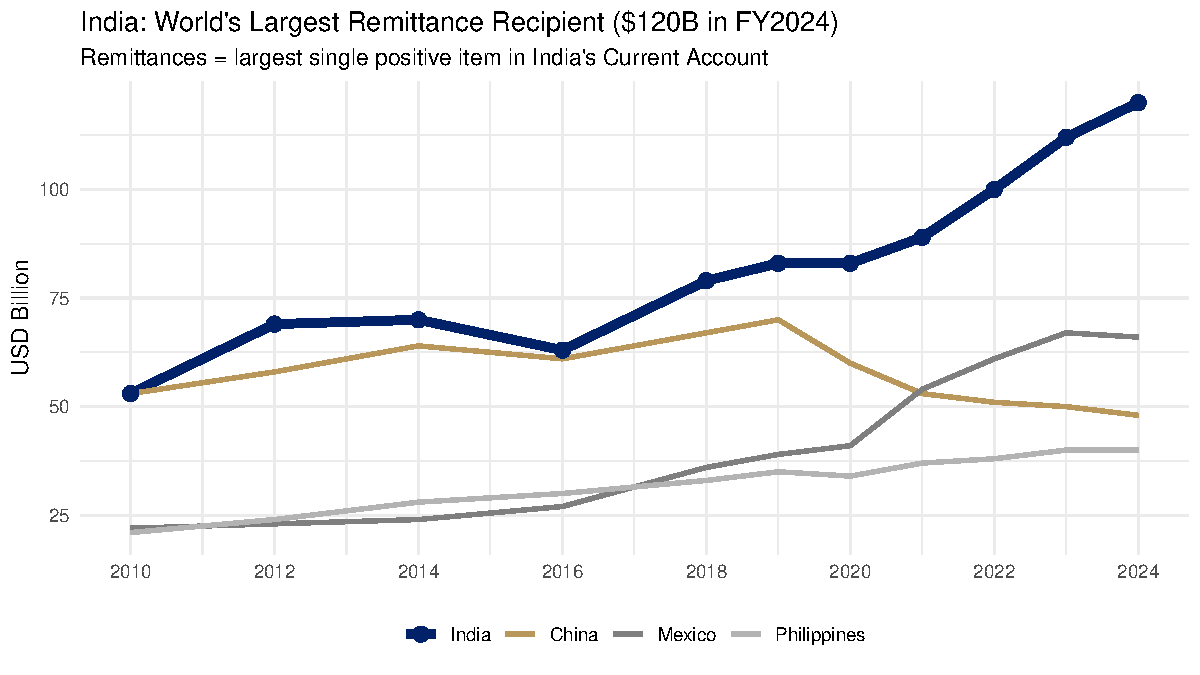
\includegraphics[keepaspectratio]{Lecture10_India_External_Sector_files/figure-beamer/fig-remittances-1.pdf}}

}

\caption{India: World's Largest Remittance
Recipient (USD billion, 2010--2024) Source: World Bank, Migration and
Remittances Data.}
\label{fig-remittances}

\end{figure}%

\textbf{Gulf concentration risk:} \textasciitilde55\% of India's
remittances come from Gulf Cooperation Council (GCC) countries. Oil
price slumps → Gulf construction slowdowns → remittance drops → India's
CAD widens. The 1991 crisis featured exactly this channel.
\end{frame}

\begin{frame}{Foreign Direct Investment (FDI) Flows}
\phantomsection\label{foreign-direct-investment-fdi-flows}
\textbf{FDI inflows FY2024: \textasciitilde\$71 billion (gross)}

\begin{columns}[T]
\begin{column}{0.55\linewidth}
\textbf{Top recipient sectors:}

\begin{itemize}
\tightlist
\item
  IT \& software: \textasciitilde\$18B
\item
  Financial services: \textasciitilde\$9B
\item
  Pharmaceuticals: \textasciitilde\$7B
\item
  Telecom: \textasciitilde\$6B
\item
  \textbf{Agriculture \& food processing: \textasciitilde\$3.6B}
\end{itemize}
\end{column}

\begin{column}{0.45\linewidth}
\textbf{Agri FDI: \$3.6B and growing}

Focus areas: - Cold chain infrastructure - Food processing (100\% FDI
allowed) - AgriTech startups - Contract farming/supply chains
\end{column}
\end{columns}

FDI in agri-food is growing but remains a small fraction --- India's
farm sector still heavily domestic-capital-driven.
\end{frame}

\begin{frame}{Forex Reserves: India's Financial Buffer}
\phantomsection\label{forex-reserves-indias-financial-buffer}
\textbf{India's Foreign Exchange Reserves --- FY2024: \$645 billion}

\textbf{Components of forex reserves:}

\begin{longtable}[]{@{}ll@{}}
\toprule\noalign{}
Component & USD B \\
\midrule\noalign{}
\endhead
Foreign currency assets (FCA) & \$571 \\
Gold & \$53 \\
SDR holdings (IMF) & \$18 \\
Reserve tranche position (IMF) & \$3 \\
\bottomrule\noalign{}
\end{longtable}

\textbf{Import cover: \textasciitilde11 months} --- well above the
conventional safe threshold of 3 months. This gives India significant
resilience against external shocks.
\end{frame}

\begin{frame}{India's 1991 Balance of Payments Crisis}
\phantomsection\label{indias-1991-balance-of-payments-crisis}
\begin{columns}[T]
\begin{column}{0.6\linewidth}
\textbf{The Crisis:}

\begin{itemize}
\tightlist
\item
  By early 1991, reserves fell to \textbf{\$1 billion} (\textless{} 2
  weeks of imports)
\item
  Iraq-Kuwait war raised oil import bill
\item
  Gulf remittances fell sharply
\item
  Fiscal deficit had grown unsustainably
\item
  Credit rating downgrades; capital flight
\end{itemize}

\textbf{India's Response:}

\begin{itemize}
\tightlist
\item
  IMF bailout loan (\$2.2B)
\item
  Gold pledged as collateral (47 tonnes)
\item
  Two-step rupee devaluation (25\%)
\item
  Structural adjustment → liberalization reforms
\end{itemize}
\end{column}

\begin{column}{0.4\linewidth}
\textbf{1991 as a turning point}

The crisis forced India to:

\begin{itemize}
\tightlist
\item
  Open up to FDI
\item
  Dismantle import licensing
\item
  Devalue rupee
\item
  Phase out industrial licensing
\end{itemize}

Agricultural trade also liberalized --- QRs on agri imports phased out
by 2001 (WTO bound).
\end{column}
\end{columns}
\end{frame}

\begin{frame}{Current Account Sustainability}
\phantomsection\label{current-account-sustainability}
\textbf{Current Account Deficit (CAD) FY2024: approximately −0.7\% of
GDP}

\textbf{India's CAD trend:}

\begin{longtable}[]{@{}lll@{}}
\toprule\noalign{}
Year & CAD (\% GDP) & Assessment \\
\midrule\noalign{}
\endhead
FY2012 & −4.8\% & Dangerously high \\
FY2019 & −2.1\% & Elevated \\
FY2022 & −1.7\% & Moderate \\
FY2023 & −2.0\% & Moderate \\
\textbf{FY2024} & \textbf{−0.7\%} & \textbf{Comfortable} \\
\bottomrule\noalign{}
\end{longtable}

A CAD of −0.7\% GDP is considered sustainable. The ``safe zone'' is
generally under −3\% for an economy of India's size and growth rate.
\end{frame}

\begin{frame}{The Edible Oil Vulnerability: A Policy Case Study}
\phantomsection\label{the-edible-oil-vulnerability-a-policy-case-study}
\begin{columns}[T]
\begin{column}{0.55\linewidth}
\textbf{The structural problem:}

India produces \textasciitilde10 million tonnes of edible oil
domestically but consumes \textasciitilde24 million tonnes.

The \textbf{14 million tonne import gap} = \$14B foreign exchange
outflow annually.

\textbf{Source concentration risk:} - 90\% of palm oil from Malaysia \&
Indonesia - Subject to export bans, price manipulation, climate shocks
\end{column}

\begin{column}{0.45\linewidth}
\textbf{Policy responses:}

\begin{enumerate}
\tightlist
\item
  \textbf{PM KUSUM} --- promote oilseed cultivation
\item
  \textbf{National Mission on Edible Oils (Oilpalm)} --- expand domestic
  oil palm to NE states
\item
  \textbf{Import duty manipulation} --- lower duties during inflation
\item
  \textbf{Buffer stock policy} --- proposed but not implemented
\end{enumerate}
\end{column}
\end{columns}
\end{frame}

\begin{frame}{Rice Export Restrictions: A Policy Dilemma}
\phantomsection\label{rice-export-restrictions-a-policy-dilemma}
\begin{columns}[T]
\begin{column}{0.6\linewidth}
\textbf{August 2023: India bans non-basmati white rice exports}

\textbf{Rationale:} - Domestic rice prices rising - Food security
concerns ahead of state elections - Erratic monsoon raised supply
uncertainty

\textbf{Impact:} - India's rice exports fell sharply (India = 40\% of
global rice trade) - Global rice prices surged 30--40\% - Indonesia,
Philippines, West Africa faced food price spikes - India's agri export
earnings fell by billions
\end{column}

\begin{column}{0.4\linewidth}
\textbf{The trade-off:}

\begin{longtable}[]{@{}ll@{}}
\toprule\noalign{}
Restrict exports & Let exports flow \\
\midrule\noalign{}
\endhead
Lower domestic prices & Higher farmer income \\
Better food security & Better forex earnings \\
Harms trading partners & Global price stability \\
\bottomrule\noalign{}
\end{longtable}

\emph{Classic food security vs.~trade earnings dilemma --- central to
agri trade policy}
\end{column}
\end{columns}
\end{frame}

\begin{frame}{India's Balance of Payments: Summary Picture}
\phantomsection\label{indias-balance-of-payments-summary-picture}
\textbf{BoP Current Account FY2024 (approximate):}

\begin{longtable}[]{@{}ll@{}}
\toprule\noalign{}
Item & USD B \\
\midrule\noalign{}
\endhead
Merchandise exports & +437 \\
Merchandise imports & −677 \\
\textbf{Trade balance} & \textbf{−240} \\
Services exports & +338 \\
Services imports & −167 \\
\textbf{Services balance} & \textbf{+171} \\
Primary income (net) & −32 \\
Secondary income (remittances) & +120 \\
\textbf{Current Account Balance} & \textbf{\textasciitilde−17} \\
\bottomrule\noalign{}
\end{longtable}

CAD of \textasciitilde\$17B on a GDP of \textasciitilde\$3.4 trillion =
about −0.5\% to −0.7\% GDP. Healthy and sustainable.
\end{frame}

\begin{frame}{India's Global Trade Rankings}
\phantomsection\label{indias-global-trade-rankings}
\textbf{India's position in global trade (WTO 2024):}

\begin{columns}[T]
\begin{column}{0.5\linewidth}
\textbf{Merchandise trade:} - Exports: \textbf{17th largest globally} -
Imports: \textbf{10th largest globally} - Share of world trade:
\textasciitilde1.8\%

\textbf{Services trade:} - Services exports: \textbf{7th globally} - IT
services: \textbf{Largest global exporter}
\end{column}

\begin{column}{0.5\linewidth}
\textbf{Agriculture specifically:} - Rice: \textbf{\#1 global exporter}
(40\% share) - Spices: \textbf{Top 3 globally} - Cotton: \textbf{Top 3
globally} - Seafood: \textbf{Top 10 globally}

India punches above its weight in agricultural exports relative to its
overall merchandise trade share.
\end{column}
\end{columns}
\end{frame}

\begin{frame}{Structural Challenges in India's External Sector}
\phantomsection\label{structural-challenges-in-indias-external-sector}
\textbf{Key vulnerabilities:}

\begin{enumerate}
\item
  \textbf{Energy import dependence} --- crude oil \$232B; geopolitical
  risk
\item
  \textbf{Edible oil import dependence} --- \$14B; food inflation risk
\item
  \textbf{Electronic goods deficit} --- \$80B; reflects low domestic
  manufacturing
\item
  \textbf{Gold demand} --- \$47B; compresses CAD but reflects domestic
  saving patterns
\item
  \textbf{China trade deficit} --- \textasciitilde\$85B; supply chain
  dependency
\end{enumerate}

\note{\textbf{Structural strengths:}

\begin{enumerate}
\tightlist
\item
  IT services surplus --- \$220B
\item
  Remittances --- \$120B
\item
  Pharmaceutical exports --- \$27B
\item
  Agricultural surplus --- +\$15.5B
\item
  Large, diversified economy --- natural hedge
\end{enumerate}}
\end{frame}

\begin{frame}{Agricultural Sector's Role in India's External Sector}
\phantomsection\label{agricultural-sectors-role-in-indias-external-sector}
\textbf{Agriculture in India's external sector: 3 key roles}

\textbf{1. Forex earner:} \$43.7B in exports --- supports BoP, provides
farmer income linkage to global prices

\textbf{2. Forex user:} \$28.2B in imports --- edible oils and pulses;
food security imperative but forex cost

\textbf{3. Policy instrument:} Government uses export/import
restrictions to manage domestic food prices --- with global spillover
effects (India = swing supplier in rice, sugar, onions)

The net surplus of \$15.5B means agriculture is a \textbf{net
contributor} to India's BoP --- a valuable buffer.
\end{frame}

\begin{frame}{Looking Ahead: India's External Sector Goals}
\phantomsection\label{looking-ahead-indias-external-sector-goals}
\textbf{India's trade policy objectives (2025--2030):}

\begin{itemize}
\tightlist
\item
  Merchandise exports target: \textbf{\$1 trillion by FY2030}
\item
  Agricultural export target: \textbf{\$100 billion by 2030}
\item
  Increase oilseed domestic production (reduce \$14B import bill)
\item
  Value-added processed food exports
\item
  Agri-GI tags to premium global markets
\end{itemize}

\note{\textbf{Structural shifts underway:}

\begin{itemize}
\tightlist
\item
  Electronics exports: \$300B (replace imports)
\item
  RCEP exit (2019) --- protected domestic agri
\item
  FTA with UAE (2022) --- agri market access
\item
  FTA with Australia (2022) --- pulses imports
\item
  FTA with UK (pending) --- key agri market
\item
  EU FTA (ongoing) --- GI products, SPS issues
\end{itemize}}
\end{frame}

\begin{frame}{Key Takeaways --- Lecture 10}
\phantomsection\label{key-takeaways-lecture-10}
\textbf{Five things to remember:}

\begin{enumerate}
\item
  \textbf{India's merchandise trade deficit is \$76B} but is more than
  offset by services surplus (\$171B) and remittances (\$120B)
\item
  \textbf{Agriculture contributes a net surplus of \$15.5B} --- making
  it a positive contributor to the BoP
\item
  \textbf{Edible oil imports (\$14B) are India's single largest
  agricultural vulnerability} --- a structural food security and forex
  risk
\item
  \textbf{India is the world's largest rice exporter} --- and unilateral
  export restrictions have significant global price consequences
\item
  \textbf{Forex reserves at \$645B (11 months import cover)} provide
  substantial external sector resilience; a far cry from the 1991 crisis
\end{enumerate}
\end{frame}

\begin{frame}{Next Lecture: Foreign Exchange Rates and Determination}
\phantomsection\label{next-lecture-foreign-exchange-rates-and-determination}
\textbf{Lecture 11 (July 7, 2026):} \emph{Foreign Exchange --- Rates and
Determination}

We will cover:

\begin{itemize}
\tightlist
\item
  What is the exchange rate and why does it matter?
\item
  Nominal vs.~real exchange rate
\item
  PPP theory and why the rupee ``should'' depreciate
\item
  Covered and uncovered interest parity
\item
  How exchange rates affect agricultural exporters and importers
\end{itemize}

\note{\begin{itemize}
\tightlist
\item
  History of India's rupee (1947 → today)
\end{itemize}

Today's external sector data (the flows --- exports, imports,
remittances) determine \textbf{tomorrow's exchange rate.} Understanding
the rate is the next step to understanding how agri trade prices are
actually set.}
\end{frame}

\section{Appendix}\label{appendix}

\begin{frame}{Additional Resources}
\phantomsection\label{additional-resources}
\begin{columns}[T]
\begin{column}{0.5\linewidth}
\textbf{Further Reading}

\begin{itemize}
\tightlist
\item
  \emph{International Economics} --- Salvatore (Ch. 13-14)
\item
  \emph{International Economics} --- Appleyard \& Field (Ch. 13-14)
\item
  RBI/DGCI\&S/APEDA databases for latest data
\end{itemize}
\end{column}

\begin{column}{0.5\linewidth}
\textbf{Key Data Sources}

\begin{itemize}
\tightlist
\item
  DGCI\&S: India's merchandise trade
\item
  RBI: Balance of payments data\\
\item
  APEDA: Agricultural export statistics
\item
  WTO: Tariff and trade databases
\end{itemize}
\end{column}
\end{columns}
\end{frame}




\end{document}
